\documentclass[border=0.2cm]{standalone}
\usepackage{tikz}
\usetikzlibrary{angles,quotes}
\usetikzlibrary{calc}


\begin{document}
\thispagestyle{empty}
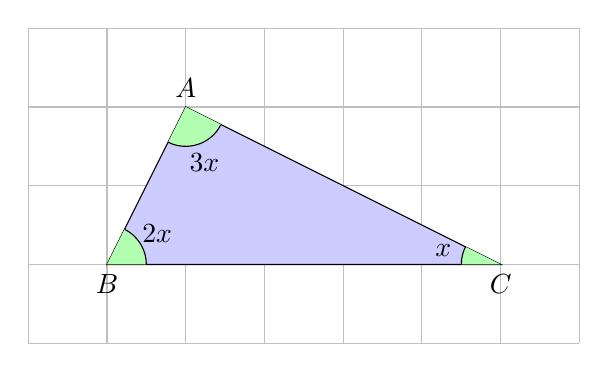
\begin{tikzpicture}

\draw[step=1,gray!50] (-1,-1) grid (6,3);

% Definindo os vértices do triângulo
    \coordinate[label=above:$A$] (A) at (1,2);
    \coordinate[label=below:$B$] (B) at (0,0);
    \coordinate[label=below:$C$] (C) at (5,0);
        
    % Desenhando o triângulo
    \draw[fill=blue!20] (A) -- (B) -- (C) -- cycle;
    
    % Marcando os ângulos internos
    \draw pic[draw, fill=green!30, angle radius=0.5cm,angle eccentricity=1.5,"$2x$"] {angle=C--B--A};
    \draw pic[draw, fill=green!30, angle radius=0.5cm,angle eccentricity=1.5,"$x$"] {angle=A--C--B};
    \draw pic[draw, fill=green!30, angle radius=0.5cm,angle eccentricity=1.5,"$3x$"] {angle=B--A--C};

\end{tikzpicture}

\end{document}
